\documentclass[11pt]{article}\usepackage[]{graphicx}\usepackage[]{color}
% maxwidth is the original width if it is less than linewidth
% otherwise use linewidth (to make sure the graphics do not exceed the margin)
\makeatletter
\def\maxwidth{ %
  \ifdim\Gin@nat@width>\linewidth
    \linewidth
  \else
    \Gin@nat@width
  \fi
}
\makeatother

\definecolor{fgcolor}{rgb}{0.345, 0.345, 0.345}
\newcommand{\hlnum}[1]{\textcolor[rgb]{0.686,0.059,0.569}{#1}}%
\newcommand{\hlstr}[1]{\textcolor[rgb]{0.192,0.494,0.8}{#1}}%
\newcommand{\hlcom}[1]{\textcolor[rgb]{0.678,0.584,0.686}{\textit{#1}}}%
\newcommand{\hlopt}[1]{\textcolor[rgb]{0,0,0}{#1}}%
\newcommand{\hlstd}[1]{\textcolor[rgb]{0.345,0.345,0.345}{#1}}%
\newcommand{\hlkwa}[1]{\textcolor[rgb]{0.161,0.373,0.58}{\textbf{#1}}}%
\newcommand{\hlkwb}[1]{\textcolor[rgb]{0.69,0.353,0.396}{#1}}%
\newcommand{\hlkwc}[1]{\textcolor[rgb]{0.333,0.667,0.333}{#1}}%
\newcommand{\hlkwd}[1]{\textcolor[rgb]{0.737,0.353,0.396}{\textbf{#1}}}%
\let\hlipl\hlkwb

\usepackage{framed}
\makeatletter
\newenvironment{kframe}{%
 \def\at@end@of@kframe{}%
 \ifinner\ifhmode%
  \def\at@end@of@kframe{\end{minipage}}%
  \begin{minipage}{\columnwidth}%
 \fi\fi%
 \def\FrameCommand##1{\hskip\@totalleftmargin \hskip-\fboxsep
 \colorbox{shadecolor}{##1}\hskip-\fboxsep
     % There is no \\@totalrightmargin, so:
     \hskip-\linewidth \hskip-\@totalleftmargin \hskip\columnwidth}%
 \MakeFramed {\advance\hsize-\width
   \@totalleftmargin\z@ \linewidth\hsize
   \@setminipage}}%
 {\par\unskip\endMakeFramed%
 \at@end@of@kframe}
\makeatother

\definecolor{shadecolor}{rgb}{.97, .97, .97}
\definecolor{messagecolor}{rgb}{0, 0, 0}
\definecolor{warningcolor}{rgb}{1, 0, 1}
\definecolor{errorcolor}{rgb}{1, 0, 0}
\newenvironment{knitrout}{}{} % an empty environment to be redefined in TeX

\usepackage{alltt}
%Required: You must have these
\usepackage{graphicx}
\usepackage{tabularx}
\usepackage{natbib}
\usepackage{pdflscape}
\usepackage{array}
\usepackage{authblk}
\usepackage{gensymb}
\usepackage{amsmath}
%\usepackage[backend=bibtex]{biblatex}
\usepackage[small]{caption}

\setkeys{Gin}{width=0.8\textwidth}
\setlength{\captionmargin}{30pt}
\setlength{\abovecaptionskip}{10pt}
\setlength{\belowcaptionskip}{10pt}

 \topmargin -1.5cm 
 \oddsidemargin -0.04cm 
 \evensidemargin -0.04cm 
 \textwidth 16.59cm
 \textheight 21.94cm 
 \parskip 7.2pt 
\renewcommand{\baselinestretch}{1} 	
\parindent 0pt
\usepackage{setspace}
\usepackage{lineno}
\bibliographystyle{..//..//refs/bibstyles/amnat.bst}
\usepackage{xr-hyper}
\usepackage{hyperref}


\title{Ranger Outline: We will come up with a better title when we feel more grounded in the results}
\date{}
\author{Dan, Cat, Nacho and Lizzie}
\IfFileExists{upquote.sty}{\usepackage{upquote}}{}
\begin{document}
\maketitle
\section*{Figures to make:}
\begin{enumerate}
\item Climate maps for species (some in supp. too)
\item Conceptual figure illustrating why variation in forcing should impact cue use
\item Results from cheapo models
\item some comparison of North America to Europe
\item Results from inter vs. intra specific model

\end{enumerate}
\section*{Abstract}
\section*{Introduction}
\textbf{For woody plants of the temperate zone the phenology, or annual timing, of spring budburst influences a myriad of ecological processes including patterns of resource allocation \citep{}, trophic interactions \citep{} and biogeochemical cycling \citep{}.}
 Through budburst timing, woody plants balance the advantages of precocious growth resumption for resource gains with the risk of damage from late season frost \citep{}. To navigate this tradeoff, woody plants have evolved complicated networks of sensory organs, hormone signaling, and physiological responses to sense environmental cues; changes in their physical environment, that signal the arrival of appropriate conditions for resuming growth.\\

\textbf{Decades of research suggest that warming spring temperatures (forcing), cool winter temperatures (chilling) and day length (photoperiod) are primary environmental cues utilized by woody plants that determine the timing of spring phenological events \cite{}}. These studies also demonstrate the there are substantial cue-use differences among species, with some species relying more heavily on some cues over others \citep{Laube:2014aa}. As anthropogenic climate change has already driven shifts in spring phenology \citep{}, identifying these interspecific differences in cue use has emerged as a major goal of phenological research \citep{}. These differences have strong implications for both predicting the rate of phenological shifts as the climate continues to warm \citep{}, and anticipating the ecological consequences of these shifts \citep{}.

\textbf{ But the quantification of cue use difference among species offers even more---a novel opportunity to interrogate long-standing theories regarding the biology underlying cue-use difference among species.} One particular relationship that can now be examined this the relationship species' geographic ranges and phenological cue use.

Climate is the major selective force on both species' geographic ranges \citep{} and their phenology \citep{}, and therefore, it is widely assumed that phenological cue-use differences among species reflect correlate with the climate of there repsecitve ranges \citep{}. That is, a species' relative reliance on forcing, chilling and photoperiod for each species should be shaped by the unique environmental conditions across a species' geographic range.\\

This has never really been tested (say better but see \citep{Zohner:2017aa}). With the recent quantification for cue use of many species \citep{} and the accessibility of high resolution climate data it is now possible to rigorously test this theory with data. Below, we briefly review the specific assumptions and predictions presented in the literature about the relationship between phenological cue-use and species' range characteristics. We then test these predictions using Bayesian models for a large suite of temperate woody species from North America and Europe.


\subsection*{Assumptions and predictions for the relationship between the cue-use and species' ranges}

Current understanding of the evolution of phenological cues assume that forcing is the prodominant cue. In this framework,a secondary reliance on photoperiod and/or chill cues evolve when forcing alone is not a reliable cue of safe growing condition \citep{Korner:2010aa}. Forcing is is an unreliable cue when patterns of forcing are unstable in the spring time. In other words when forcing is variable.When considered at the macro-ecological scale, this conceptual framework predicts species with high variation in forcing in there range should have a stronger response to chilling and or photoperiod and a weaker sensitivity to forcing. Here after, we refer to this as the range-cue use hypothesis\\

An implicit assumption the range-cue use hypothesis is that among species cue variation is higher than within speices (ie cue use is ``conserved" at the species level). If rather, cue use patterns are locally adapted, the range-cue use hypothesis would not hold. There is not yet a strong consensus about to whar degree cue use is locally adapted and it likely varies between phenophases \citep{}, and organisms \citep{}. As such, any analysis considering species ranges and cue use must account for intra-specific differeneces as well.

A major hurdle for testing the range cue-use hypothesis is that, when considered in the context of a species' geographic range, forcing variation occurs on multiple temporal and spatial scale.
\begin{enumerate}
\item Intra-annual variation (Temp.var ggdlf)
\item Inter-annual (cite Zohner) (Temp.var stv)
\item local cliamte variation (Geo.var ggdlf)
\item Deeper time stability \citep{} (literature)
\item global climate varaition (continents). In general NA is more variable than Europe
\end{enumerate}

 Any of these level of varation could itself drive selecion for secondary cue usage (photoperiod/chilling) and it is unclear how they interact or which is most important \citep{Zagmajster:2014aa}. Understanding the relationships between spring forcing variation at multiple spatio-temporal scales is a second key to robustly testing the range-cue use hypothesis.

A possible alternative method that avoids this issue is to consider the realtionship between range sizes and cue use. Rapoport's rule, a long established concept in biogeography suggest that species ranges should be larger closer to the poles \citep{}. The proposed mechanism underlying this pattern is increased climatic heteregineity selects for larger range sizes \citep{}. While Rapoport's rule does not explictly address climate hetergenity in the early spring (the time relevant to leaf phenology), its general logic has been evoked to explain cue use patterns \citep{} and been broadly observed for temperate trees of North America \citep{}. However, it is unclear how generalizable Rapoports rule is \citep{Gaston:1999aa} and its relevance to spring phenological cues should be tested explicitly.\\

\textbf{Predictions}\\
For these theoretical frameworks we can make several predictions regarding the range-cue use hypothesis:\\
\begin{enumerate}
\item More STV or variation in GGD2lf should increase chill and photo sensitivity. Decrease forcing sensittivity. (First principles)
\item North America should increase chill and photo sensitivity. Decrease forcing sensitivity.
\item Larger ranges should correlate with increase chill and photo sensitivity. Decrease forcing sensittivity. (Rapoport)
\item More northern ranges should correlate with increase chill and photo sensitivity. Decrease forcing sensittivity. (Rapoport)
\end{enumerate}

We tested these underlying assumptions aboutt he relationship between climate variables in a species ranges and specific predictions for the relationship between range climate and cue use using the OSPREE database, and climate data, and models. Our interrogation of these relationships between climate and cue use not only clarifies the evolutionary drivers of cue use, but offers new insights regarding implications of climate change as both species' ranges and phenology continue to shift with warming.

\section*{Methods}
\subsection*{Phenological data and cue-use estimates}
Dan and/or Lizzie write:
\begin{itemize}
\item Introduce OSPREE
\item Species selection
\item Model description
\end{itemize}

\subsection*{Species' range characteristics}
Cat and/or Nacho write?\\
\begin{itemize}
\item Climate data \textbf{(Figure of range maps with one climate variable, other could go to supplement)}
\item note on temp vs. geographic variation
\item calculation of GDD last frost
\item STV
\item range area
\end{itemize}


\subsection*{Statistical analysis}
\subsubsection*{Intra vs. interspecific models}
Cat or Lizzie or Dan write

\subsubsection*{Range-climate correlations}
Correlation coefficents for NA and EU (basically how we made fig \ref{fig:climcor} )


\subsubsection*{Secondary cue use}
Dan write description of ``Sequential modeling".\\
Dan write about continent comparisions.\\

\section*{Results}
\subsection*{Intra vs. interspecific}
We found that inter-specific variation in cue us was higher than intraspecific.
\subsection*{Coherance of forcing variation}
\begin{enumerate}
\item Good corelation between spatial and temporal intra-annual variability (Fig \ref{fig:climcor} a)
\item Decentcorelation between inter and intra-annual variability in North America but not in Europe  (Fig \ref{fig:climcor} b,c)
\item Also please note the magnitude of variation between NA and Europe is quite different.
\end{enumerate}

\subsection*{Rapoports Rule in spring climate variability}
\begin{enumerate}
\item Basic prediction (increase latitude correlated with larger ranges) of Rapoports Rule is met for our species subset (Fig \ref{fig:climcor} d,e)
\item Predictions about range size and variability of cliamte varaible not well supported
(Fig \ref{fig:climcor} f-j though okay for STV in Europe pannel h,i)
\end{enumerate}


\subsection*{Climate variation and secondary cue use}
\begin{itemize}
\item mu plot for STV,ggglftemp and ggdlfgeo.
\item Area by cue. centroid by cue.
\item Discuss differences between NA and EU in above plots and that overall, North America does have stronger secondary cue use (Fig \ref{fig:conts}) 
\end{itemize}
\section*{Discussion}
Things to address in the discussion:
\begin{enumerate}
\item Why differences between NA and EU show up for correlation between temp and geo variation, and STV and range area. (perhaps this is where we can talk about the artifact of STV not capturing ``biological spring" across a large range)
\item In general why these continents show different trends
\item Not surprised we dont see Rapaports rule strongly. It's not so well supported in general \citep{Gaston:1998aa}
\item Alterntaive explainations: A ton of hypotehses about community dynamics, phylogeny etc


\bibliography{..//..//refs/ranges}

\section*{Figures}
\begin{figure}[h!]
    \centering
 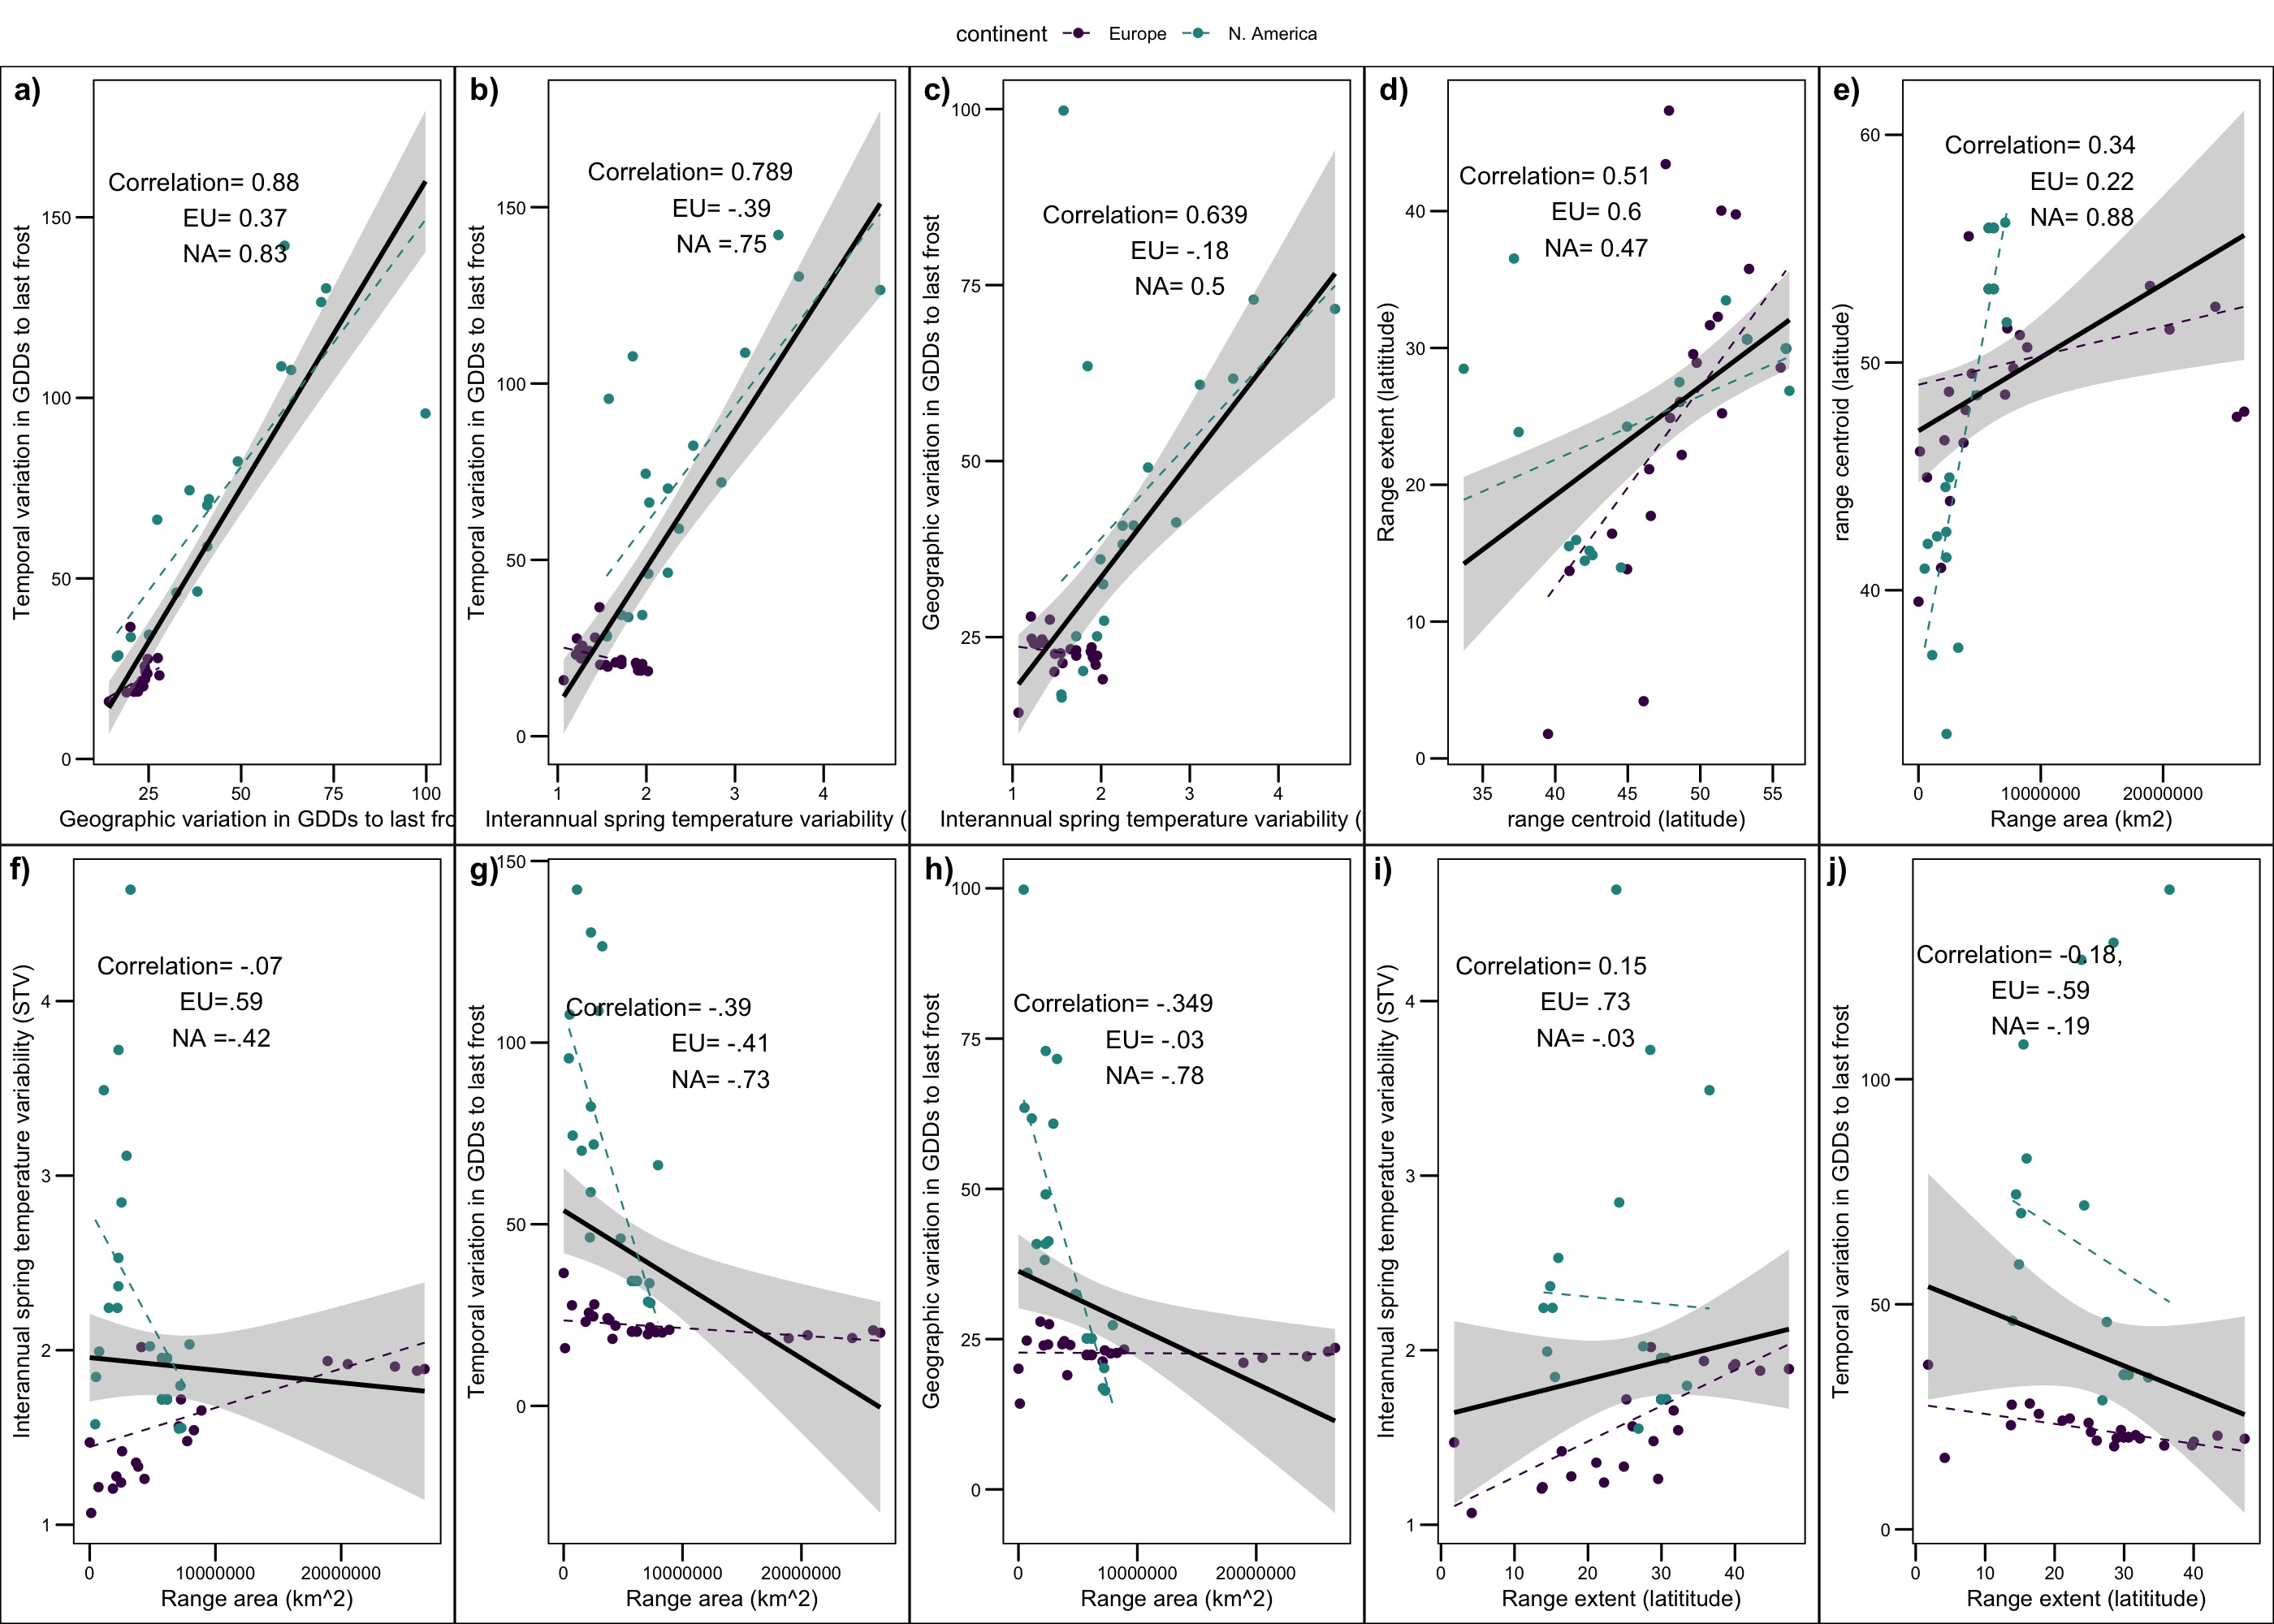
\includegraphics[width=\textwidth]{..//..//analyses/ranges/figures/clim_params.jpeg} 
    \caption{Correlations between levels of forcing variation. }
    \label{fig:climcor}
\end{figure}

\begin{figure}[h!]
    \centering
 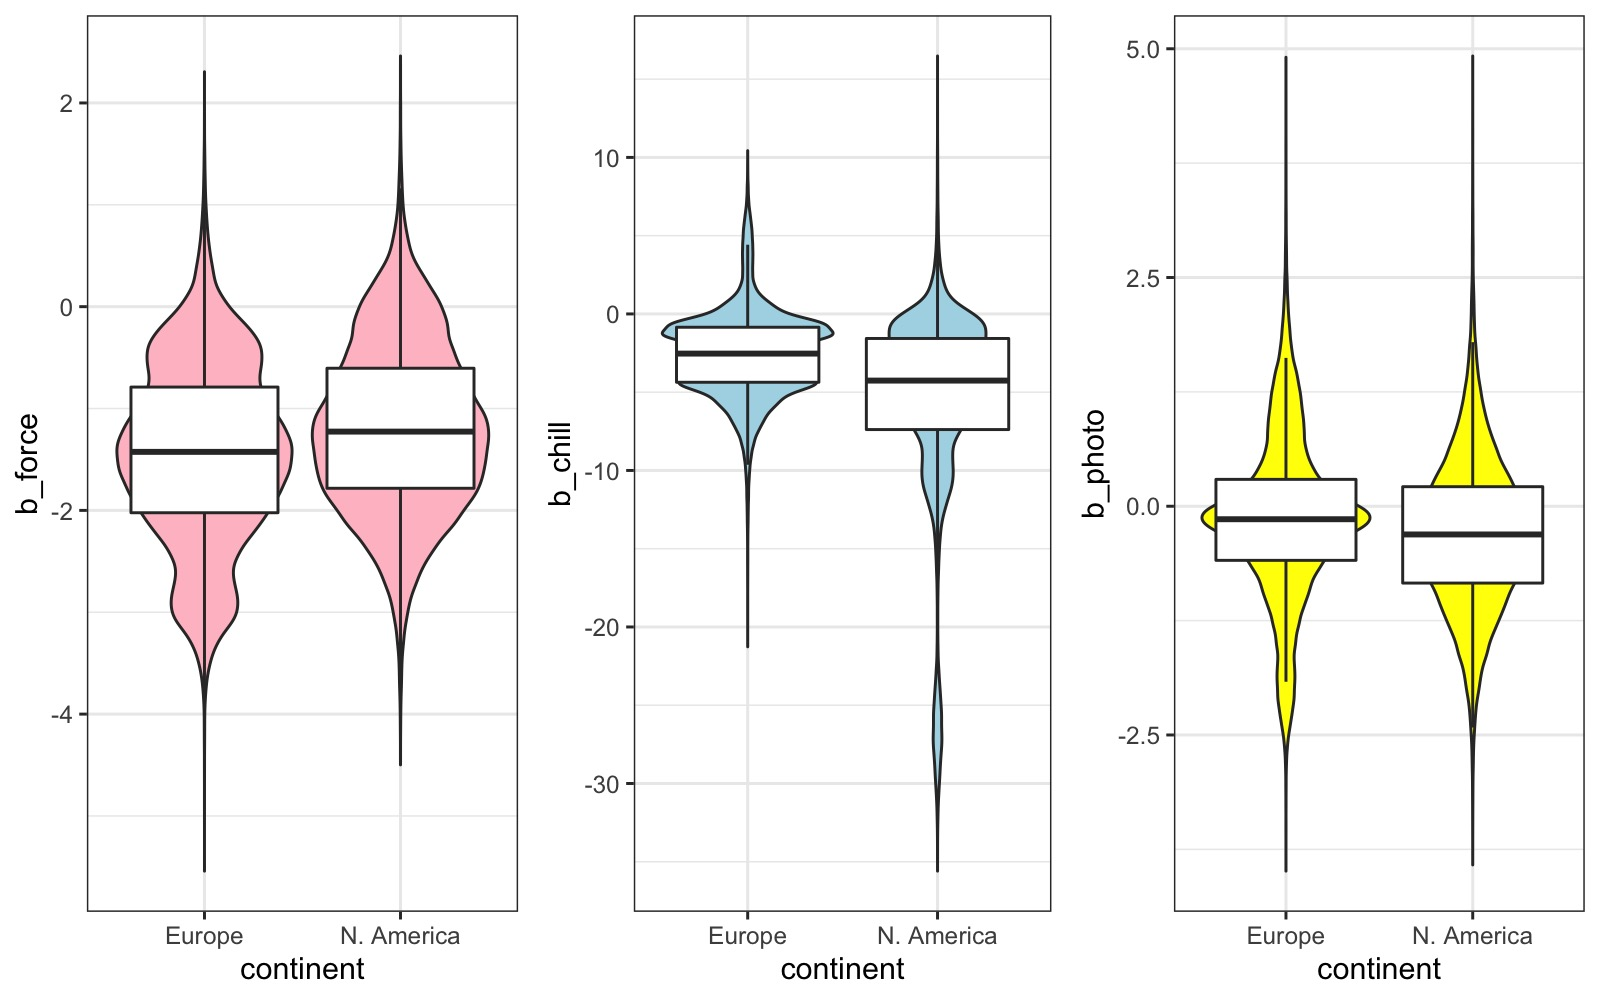
\includegraphics[width=\textwidth]{..//..//analyses/ranges/figures/continental_cues.jpeg} 
    \caption{North American species which experience high spring forcing variation have stronger (more negative) chilling and photoperiod sensitivity and weaker (less negative) forcing sensitivity than European speccies. This is based on posertior estimates for each species grouped by continent}
    \label{fig:conts}
\end{figure}


\end{document}
